\documentclass{article}
\usepackage[utf8]{inputenc}
\usepackage{custom}

\title{INMA 2361 - Nonlinear dynamical systems \\
        Project : Language dynamics}
\author{Quentin Lété}
\date{January 2018}

\begin{document}

\maketitle

\section{Introduction}
Languages death is a major cultural issue on our planet.
On the aprroximately 7,000 languages in the world, more than half of them are endangered.
It is estimated that one language is dying every two weeks.
90 \% of the languages are expected to disappear with the current generation \cite{death}.
In this context, it is important to come up with models to explain this death so that policies can be adapted.
Many models focused on the properties of the languages like grammar or syntax were developed.
Here we restrict ourselves to the mathematical models in the framework of dynamical systems. \\
Abrams and Strogatz explained in \cite{death} how the death of a language competing with another can be explained with a very simple model.
Other authors (\cite{bilingual}) have extended this model to account for the possibility of bilinguism among the population. In particular, they show when coexistence is possible.
In this work, I propose to extend the two previous models to model the temporal change on the perception of a language when it is endangered.
I will also analyse numerically some spatial properties of the dynamics and test on a real dataset for the Irish case.
As the model developed here is a direct extension of \cite{bilingual} and as a comprehensive state space analysis was made in that paper,
I will in each section recall and explain the important results found in \cite{bilingual} before extending to the new temporal and spatial considerations. \\
The report will be organised as follows : in section \ref{sec:basic},
I will prensent the equations of the models proposed by \cite{death} and \cite{bilingual} and define the notations used.
Section \ref{sec:1d} will describe the extension of the model proposed for the change in the perceived status of a language and apply it to extend the Abrams-Strogatz model.
Section \ref{sec:2d} will do the same for \cite{bilingual}.
Section \ref{sec:spatial} will analyse some spatial properties of the system.
Section \ref{sec:conclusion} will be the conclusion of this project.

\section{Basic models and notation}
\label{sec:basic}
We consider a system of two competing languages X and Y.
Abrams and Strogatz made the assumption that the attractiveness of a language depends on two things : its number of speakers and its perceived status.
The perceived relative status, denoted by $s \in [0;1]$ is the perceived social or economical advantage that one has when one speaks this language.
We denote by $x$ and $y$ the normailized population of speakers of language X and Y, i.e. $x+y=1$. $P_{YX}(x, s)$ is the probability per unit of time that a Y speaker becomes an X speaker. As stated above, it is a function of both $x$ and $s$.
A simple model for the evolution of this system is
\begin{equation}
\label{eq:1dsimple}
\dx = yP_{YX}(x, s) - xP_{XY}(x, s)
\end{equation}
which, as $y = 1-x$, is a 1D system. \\
By interchangability of the two languages, one should have that $P_{XY}(x, s) = P_{YX}(1-x, 1-s)$. Abrams and Strogatz proposed the following function for the probability of switching of language :
\[ P_{YX}(x,s) = cx^as \hspace{1cm} P_{XY}(x,s) = c(1-x)^a(1-s) \]

Abrams and Strogatz empirically determined that the parameter $a$ is quite constant trough many populations, with a mean of $1.31$ on a standard deviation of $0.25$. The parameter $s$ has to be estimated for each separate case. \\

This model doesn't account for the possibility of existence of a bilingual population.
In some cases, this population plays an important role for the persistence of a language.
A model taking a bilingual population into account was first proposed in \cite{BAGGS19939}.
The idea is to introduce a bilingual population $b$ such that $x+y+b=1$.
They also introduce a parameter $k \in [0;1]$ describing the similarity between the two languages.
If $k = 1$, $Y = X$ whereas if $k = 0$, the languages are totally different.
By simply extending the previous model, we obtain the following equations

\begin{equation}
\label{eq:bil}
\begin{cases}
\dx = yP_{YX} + bP_{BX} - x(P_{XY} + P_{XB}) \\
\dy = xP_{XY} + bP_{BY} - y(P_{YX} + P_{YB}) \\
\db = xP_{XB} + yP_{YB} - b(P_{BX} + P_{BY}) \\
\end{cases}
\end{equation}
with the following transition functions :

\[
\begin{cases}
P_{XB} = c \cdot k (1-s) (1-x)^a \\
P_{YB} = c \cdot k s (1-y)^a \\
P_{BX} = P_{YX} = c \cdot (1-k) s (1-y)^a \\
P_{BY} = P_{XY} = c \cdot (1-k) (1-s) (1-x)^a \\
\end{cases}
\]

This model was validated by the authors who found that it fits correctly the historical data of the evolution of speakers in the case of Galician and Spanish for a value of $k = 0.8$. \\
In \cite{BAGGS19939}, some theoretical results are given about the possibility of coexistence. It is shown that coexistence is indeed possible. In \cite{bilingual}, they are interested in the range of values of $s(k)$ that leads to coexistence. This is done using bifurcation theory. In particular, it is first shown that the system expereinces a subcritical Pitchfork bfurcation when $s = \frac{1}{2}$. For the general case $s \ne \frac{1}{2}$, there is also a bifurcation but this time, it is a saddle-node bifurcation. Before a critical value of $k$, the system has one fixed point whereas after, it has three fixed point, one of them being stable. This proves that coexistance is possible.

\section{One dimensional temporal extension}
\label{sec:1d}
In this section, we wish to present an extension of the system (\ref{eq:1dsimple}) to take into account the evolution of the perveiced status $s$.
We extend slightly this notion of status to other factors that can make a person want to learn the language, like the cultural factor.
Indeed, in many cases, the very fact that a regional language is endangered increase its status among the population.
The Irish language is a good example.
When Irish people realised that the possibility of extinction of their language existed, people startded to consider it differently.
Policies were established to make the language mandatory at school and it gained a lot of influence so that it became primary to know Irish to be able to be accepted in high ranked colleges or apply to some jobs.
Even closer to us, in Wallonia, one can argue that its decrease in popularity was followed by a small but real increase in its status thanks among other to cultural policies or independent actions.
Moreover, the models described in \cite{death} or \cite{bilingual} aim to help to develop policies.
These policies will often lead to an increase in the status $s$ and it would thus be intereting to have a model where $s$ eveloves dynamically. \\
Modelling this phenomenon can be done by considering a non-stationary $s$. The system (\ref{eq:1dsimple}) would become

\begin{equation}
\label{eq:1dtemp}
\begin{cases}
\dx = c\big( (1-x)sx^a - x(1-s)(1-x)^a \big) \\
\ds = S(x, s) \\
\end{cases}
\end{equation}

where the function $S(x,s)$ will model the dynamics of $s$ and need to be defined.
The requirements for this function are that $S(x,s)$ should be positive when $x$ is small, negative when $x$ is large and $0$ when $s = \frac{1}{2}$.
Moreover, it should be such that $s(t) \in [0;1] \hspace{0.5cm} \forall{t}$.
One function the I propose to model the dynamic of $s$ that fulfill the requirements is the following

\begin{equation}
\label{eq:sdyn}
S(x,s) = (\frac{1}{x}-\frac{1}{y})s(1-s) = (\frac{1}{x}+\frac{1}{x-1})s(1-s)
\end{equation}

The first part of the function, $\frac{1}{x}+\frac{1}{x-1}$, is there to ensure the first requirement and has the folllowing shape

\begin{figure}
\centering
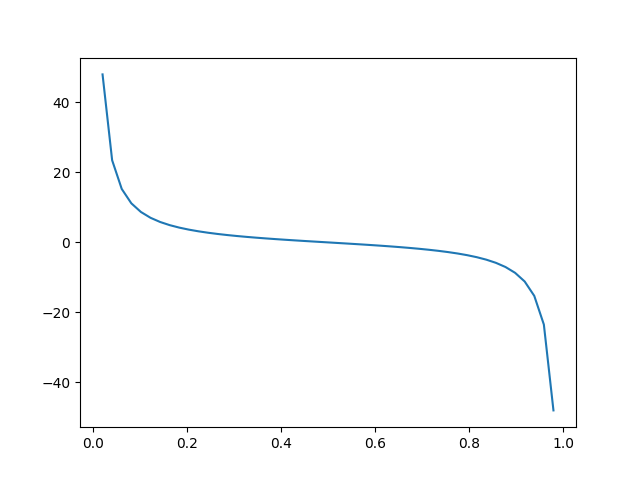
\includegraphics[scale=0.5]{functionofs.png}
\caption{Function $\frac{1}{x}+\frac{1}{x-1}$ on $[0;1]$}
\label{fig:functionofs}
\end{figure}

This function tends respectively to $-\infty$ and $\infty$ in $0$ and $1$ and is $0$ in $\frac{1}{2}$.
The second part of the function, $s(1-s)$, is added to ensure that $s$ stay in $[0;1]$.
This is proved by the following theorem. \\

\begin{theorem}{}
\label{posinv}
If $S$ is given by equation (\ref{eq:sdyn}) and if $a>0$, then the set $A = (0;1) \times [0;1]$ is positive invariant for system (\ref{eq:bil}).
\end{theorem}

\begin{proof}
We will first show that there exists four particular trajectories that correspond respectively to the four side of the square A, i.e. the side $x=0$, $x=1$, $s=0$ and $s=1$. \\
For $x=0$, as the interval on $x$ is open, we will show that we have a trajectory as close as we want to the side of the square.
Let $\epsilon_1>0$ and $\epsilon_2 >0$, there exists $\delta > 0$ and $T > 0$ such that if $x < \delta$ and  if $\epsilon_1>s_0>0$, $s(t) > 1- \epsilon_2 \, \, \forall t > T$.
Indeed, if $x = \delta$ and  if $s=1-\epsilon_1$, the system becomes
\[
\begin{cases}
\dx =  (1-\delta)(1-\epsilon_1)\delta^a - \delta\epsilon_1(1-\delta)^a  \\
\ds = (\frac{1}{\delta}+\frac{1}{\delta-1})(1-\epsilon_1)\epsilon_1 \\
\end{cases}
\]
Therefore, we have that $\underset{\delta \rightarrow 0}{\text{lim}} \dx = 0$, $\underset{\delta \rightarrow 0}{\text{lim}} \ds = \infty$ wich means that $s$ will become enventually as close as we want to $1$. By symmetry, we can use a similar argument for the side $x=1$.
When $s=0$, $\ds = 0$ and $\dx = -x(1-x)^a < 0 \, \forall{x}$ so that $x$ decreses from $1-\epsilon$ to $\epsilon$ for each $\epsilon$ and similarly for $s=1$.
This shows that there exists four particular trajectories that correspond respectively to the four sides of the square A.
Now, as the vector field is Lipshitz continuous on $A$, the existence and unicity of solutions holds.
This means that trajectories cannot cross.
Therefore, each trajectory that will start inside $A$, will stay in $A$.
\end{proof}

The system has only one equilibirum point inside $A$, the point $(\frac{1}{2}, \frac{1}{2})$.
If both language have the same status and the same number of speakers, then no language will extinct and the system will stay as such forever.
We suppose that this fixed point is unstable.
Let us verify this mathematically.
The Jacobian matrix has the following components
\[
\begin{cases}
a_{11} = sax^{a-1} - s(a+1)x^a - (1-s)(1-s)^a + a(1-s)(1-x)^{a-1} \\
a_{12} = (1-x)^a + x(1-x)^a \\
a_{21} = (-\frac{1}{x^2}-\frac{1}{(x-1)^2})s(1-s) \\
a_{22} = (\frac{1}{x}+\frac{1}{x-1})(1-2s) \\
\end{cases}
\]

If we compute the eigenvalues of A at $(\frac{1}{2}, \frac{1}{2})$ for $a=1.31$, we have indeed that
\[
\begin{cases}
\lambda_1 = 0.194602+1.08263i \\
\lambda_2 = 0.194602-1.08263i \\
\end{cases}
\]
As the real part of both eigenvalues are positive, the equilibrium is unstable. \\
We will now show that the system evolves towards a limit cycle or a closed orbit by using Poincarré-Bendixson theorem.
Let us recall this theorem. \\

\begin{theorem}{Poincarré-Bendixson}
\label{th:pb}
Let $\dx = f(x)$ be a dynamical system with $x \in \mathbb{R}^2$. Let $R$ be a closed bounded subset of $\mathbb{R}^2$ that contains no equilibrium points. Let $t\rightarrow x(t)$ be a trajectory that stays in $R$ for all $t > 0$ and suppose that $f \in C^1$ in an open subset that contains $R$.\\
Then, $x(t)$ is a periodic solution or $x(t)$ tends towards a closed orbit ad $t \rightarrow \infty$.
\end{theorem}

To apply this thoerem to our system, let $\epsilon > 0$ and let $R = A \backslash B(\epsilon;(\frac{1}{2},\frac{1}{2}))$. We have shown that $(\frac{1}{2},\frac{1}{2})$ is unstable and $A$ is positively invariant. Therefore, all trajectories satisfy the assumptions of theorem \ref{th:pb}.

\section{Temporal extension for model with bilinguism}
\label{sec:2d}

\section{Spatial analysis}
\label{sec:spatial}

\section{Conclusion}
\label{sec:conclusion}



\bibliographystyle{plain}
\bibliography{references}

\end{document}
